\newpage
\restoregeometry
\section{Implementierung}
\subsection{Softwarestack}
Die prototypische Entwicklung eines leichtgewichtigen Rich Data Interface für Copernicus-Daten erfolgte im Rahmen dieser Arbeit mit der Programmiersprache Python.
Diese ist nicht nur aufgrund ihrer Einfachheit vorteilhaft sondern erlaubt auch den Zugriff auf eine große Zahl von Packages für die unterschiedlichsten 
Anwendungsfälle. 
Weite Teile des Rich Data Interface wurden mithilfe des Flask-Frameworks umgesetzt. Dieses erlaubt das schnelle Entwickeln einer leichtgewichtigen API.  
Neben Python Standard-Bibliotheken kommen nur wenige zusätzliche Packages zum Einsatz. Um zu Anfragen passende Sentinel-1 Datensätze aus dem 
Copernicus-Access-Hub zu finden kommt das Package sentinelsat zum Einsatz. Das Herunterladen der Sentinel-1 Datensätze erfolgt ebenfalls mit diesem Package. 
Die Prozessierungen der Sentinel-1 Daten werden mit dem Package snappy durchgeführt. 
Dieses ist ein Wrapper für die SNAP Software welche im Rahmen des Copernicus-Programmes kostenlos zur Verfügung 
gestellt wird. Mit snappy lassen sich die Funktionen der Sentinel-1 Toolbox in Python verwenden. 
Statistische Auswertungen der Radarbilder werden mit dem Package skimage durchgeführt. Da die Radarbilder jedoch auch zugeschnitten und 
mathematisch zu kombinieren sind werden auch die Packages gdal, ogr und osr verwendet. 

\subsection{Struktur}
Die Anwendung ist in vier Python-Scripte aufgeteilt. Im api.py Script ist die API der Anwendung definiert. 
Die geordnete Abarbeitung der angelegten Jobs werden vom Script processing.py nach dem Modell der Queue gesteuert. 
Dies bedeutet das zeitgleich nur ein Job ausgeführt wird. Nach dessen Beendigung wird der älteste angelegte Job gewählt und bearbeitet.
Die eigentlichen Prozesse sowie 
Hilfsfunktionen befinden sich im utils.py Script. Dazu zählen auch die eigentlichen Prozesse sowie Parser für 
ihre Eingabedaten. Das test.py Script kann dazu genutzt werden um die Stabilität und Standardkonformität der API zu testen und enthält des Test-Suit.

Diese Scripte verwalten Dateien in einem einfachen Verzeichnissystem. Templates für statische Ressourcen befinden sich im Verzeichnis \textit{templates/}. HTML-Dateien 
befinden sich im Verzeichnis \textit{templates/html/} und JSON-Dateien im Verzeichnis \textit{templates/json/}. Das Unterverzeichnis \textit{templates/json/processes/} enthält die 
Beschreibungen der von der Anwendung angebotenen Prozesse. 
Die Anwendung erlaubt das persistente hinterlegen von Sentinel-1 Datensätzen um zeitaufwendiges Herunterladen zu vermeiden. Diese Datensätze können im Verzeichnis \textit{data/} abgelegt werden. Jeder Sentinel-1 Datensatz enthält eine .kml-Datei welche 
Metadaten zum Datensatz enthält. Diese werden im Unterverzeichnis \textit{data/coverage/} abgelegt. 
Jeder angelegte Job, also jede auszuführende Instanz eines Prozesses erhält ein einzigartiges Verzeichnis innerhalb des Verzeichnisses \textit{jobs/}. In diesem 
Verzeichnis befinden sich eine Status- und eine Job-Datei sowie ein weitere für die Bearbeitung des Jobs benötigte Dateien. 
Neben diesen Dateien enthält jedes Job-Verzeichnis ein Unterverzeichnis \textit{results/} in dem die Ergebnisse des jeweiligen Jobs abgelegt werden.

\begin{figure}[H]
    \centering
    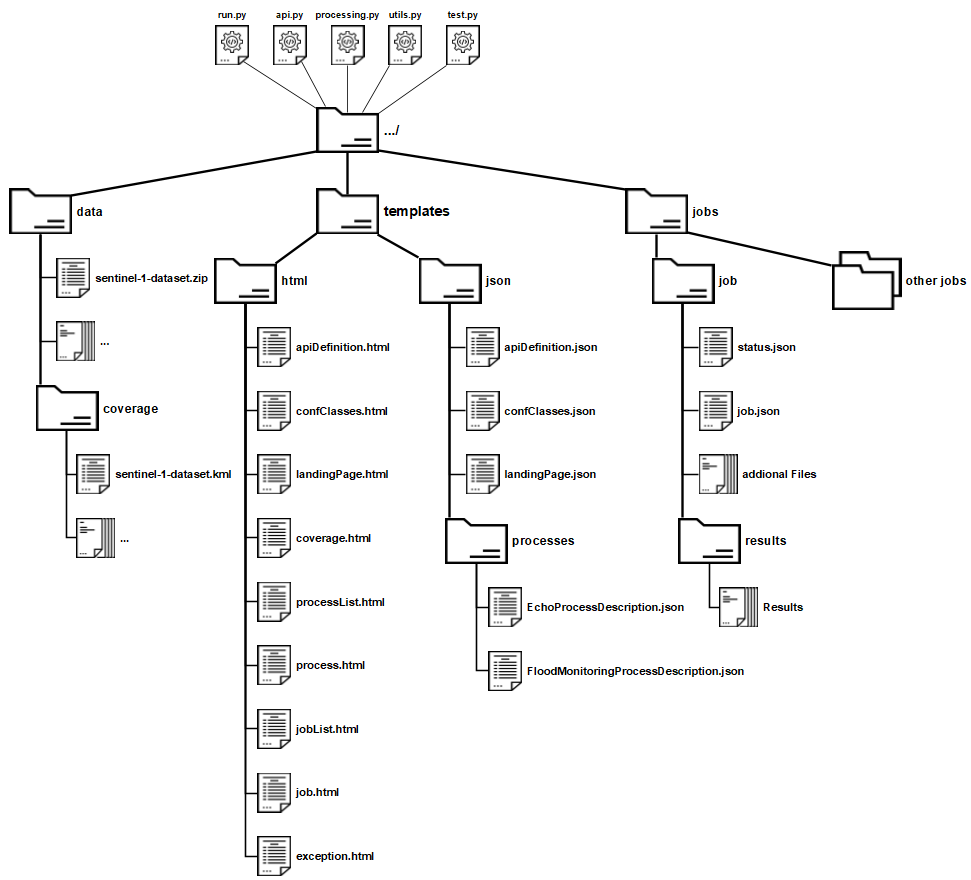
\includegraphics[width=\textwidth]{Bilder/folders.png}
    \caption{Struktur der prototypischen Implementierung \cite{structure}}
    \label{structure}
\end{figure}

Insgesamt handelt es sich bei der prototypischen Implementierung eines Rich Data Interfaces for Copernicus-Daten also um eine Anwendung welche Überschwemmungsmasken und Daten zur Hochwasseranalyse als Ressourcen bereitstellt.
Zugriff auf diese Ressourcen erhalten Nutzer über eine OGC API - Processes - Part 1: Core standardkonforme API. 

\subsection{Ressourcen}
Ressourcen sind die über die Endpoints der API bereitgestellten Informationen und Dateien. Sie können in unterschiedlichen Repräsentationen vorliegen. 
Die Ressourcen werden vom OGC API - Processes - Part 1: Core Standard mittels Schemata im .yaml-Format beschrieben. 
Diese definieren neben den Bezeichnungen für Elemente auch ihre Datentypen und ob sie optional sind oder nicht. 
Die meisten angebotenen Ressourcen können um Media-Type \textit{text/html}, also als HTML-Dateien oder im Media-Type \textit{application/json} also als 
JSON-Dateien angefragt werden. Um aus diesen Dateien einen Response zu generieren werden .html-Dateien zuvor mit der Methode \textit{render\_template()}, welcher auch 
dynamische Inhalte übergeben werden können gerendert während .json-Dateien zunächst geladen und anschließend 
mit der Methode \textit{jsonify()} bearbeitet werden. Beide genannten Methoden
geben ein Response-Objekt zurück welches zusammen mit Headern und einem HTTP-Statuscode versandt werden kann. \\

Jede Ressource enthält zudem eine Verknüpfungen zu sich selbst mit der Relation \textit{self} und gegebenenfalls eine Verknüpfung 
zur Ressource im jeweils anderen Media-Type mit der Relation \textit{alternate}. 

\subsection{Encodings}
In der Requirements Class JSON wird definiert welche Ressourcen im Media-Type \textit{application/json} angefragt werden können. Dazu gehören alle Responses der 
Endpunkte API Landing Page, API Definition, Conformance Deklaration, Prozess Liste, Prozess Beschreibung, Prozess Ausführung und Job Status welche mit dem 
HTTP-Statuscode 200 versandt werden. Da die prototypische Implementierung auch die Endpunkte Job Liste und Coverage bereitstellt können die korrespondierenden
Ressourcen auch im Media-Type \textit{application/json} angefragt werden.\\

In der Requirements-Class HTML werden analog zur Requirements Class JSON jene Ressourcen definiert welche im Media-Type \textit{text/html} angefragt werden können. Jedoch
entfällt in dieser Requirements-Class die Einschränkung auf bestimmte Endpunkte und alle Responses welche mit dem HTTP-Statuscode 200 versandt werden müssen den 
Media-Type \textit{text/html} unterstützen.\\
Stellen Endpoints ihre Ressourcen sowohl den Media-Type \textit{application/json} als auch \textit{text/html} zur Verfügung so können Nutzer diesen über den optional Parameter
\textit{f} oder \textit{content\_type} spezifizieren. Wird kein Media-Type über diese Parameter spezifiziert so wird standardmäßig der Media-Type \textit{text/html} verwendet. \\

\subsection{HTTP 1.1}
Die Umsetzung des Requirements HTTP 1.1 (RFC 2616) aus der Requirements-Class Core verlangt das die API exklusiv das HTTP 1.1 unterstützt. 
Das Flask-Framework nutzt standardmäßig das HTTP 1.0. Teil des Flask-Frameworks ist die WSGI Bibliothek Werkzeug welche
das Implementieren von Webanwendungen erlaubt. Um die verwendete HTTP-Version von 1.0 auf 1.1 umzustellen müssen Variablen 
in Werkzeug angepasst werden. Nach dem Import der Module WSGIRequestHandler und BaseWSGIServer kann in beiden die 
Version des HTTP Protokolls angepasst werden (siehe Anhang \ref{appendixconfWerkzeug}). 

In diesem Requirement werden zudem alle HTTP-Statuscodes gelistet die Nutzer von einer standardkonformen Implementierung mindestens erwarten können. 
\begin{table}[H]
    \caption{Vorgesehene HTTP-Statuscodes \cite{ogc_api_processes_core}}
    \centering
    \begin{tabular}{c c} 
        HTTP-Statuscode & Bedeutung\\ 
        \hline
        200 & OK\\
        201 & Created\\
        204 & No Content\\
        400 & Bad Request\\
        401 & Unauthorized\\
        403 & Forbidden\\
        404 & Not Found\\
        405 & Method Not Allowed\\
        406 & Not Acceptable\\
        410 & Gone\\
        429 & Too Many Requests\\
        500 & Internal Server Error\\
        501 & Not Implemented\\
    \end{tabular}\label{httpcodes}
\end{table}
Alle erfolgreichen Anfragen welche eine Resource liefern mit dem HTTP-Statuscode 200 beantwortet. Die Verwendung nicht zulässiger HTTP-Methoden resultieren 
in Antworten mit dem Status-Code 405 während Anfragen für nicht unterstütze Media-Types mit dem Status-Code 406 beantwortet werden. Kommt es zu Fehlern bei der Ausführung 
des Programmcodes antwortet die Anwendung mit dem HTTP-Statuscode 500. Werden durch eine Anfrage Ressourcen neu erzeugt oder nicht gefunden antwortet die Anwendung mit 
den HTTP-Statuscodes 201 beziehungsweise 404. Der Standard erlaubt die Nutzung weiterer HTTP-Statuscodes \cite{ogc_api_processes_core}.

\subsection{Endpoints}
\subsubsection{API Landig Page Endpoint}
Der API Landing Page Endpoints ist Teil der Requirements-Class Core.
Der Endpoint kann über den URL \textit{http://HOST:PORT/?f=<MEDIA-TYPE>} angefragt werden und liefert als Resource die 
API Landing Page (siehe Anhang \ref{SchemaLandngPageyaml}). 
Die einzig zulässige HTTP-Methode für diesen Endpoint ist die HTTP-Get Methode.\\ 
Die API Landing Page kann als Eintrittspunkt zu allen anderen Funktionalitäten der Anwendung bezeichnet werden. Sie enthält Verknüpfungen zu den Endpoints, 
API Landing Page, API Definition, Conformance, Process List, Process Description, Job List und Coverage.\\
Die API Landing Page kann in den Media-Types \textit{text/html} (siehe Anhang \ref{RessourceLandingPageHTML}) und \textit{application/json} 
(siehe Anhang \ref{RessourceLandingPageJSON}) abgerufen werden. \\

Ein an den API Landing Page Endpoint gerichteter Request wird zunächst auf die verwendetet HTT-Methode hin überprüft. Handelt es sich nicht um die HTTP-Get 
Methode wird der HTTP-Statuscode 405 als Response versandt. Im nächsten Schritt erfolgt die Prüfung des angefragten Media-Types. Enthält der Parameter \textit{f} 
oder der Parameter \textit{content\_type} einen nicht unterstützten Media-Type wird als Response der HTTP-Statuscode 406 versandt. Wird der Media-Type nicht spezifiziert oder
\textit{text/html} angefragt wird die landingPage.html an die Funktion an den Renderer übergeben um ein Response-Objekt zu erzeugen. Spezifiziert der Request 
den Media-Type \textit{application/json} wird das Response-Objekt aus der landingPage.json erzeugt. Dieses wird mit dem HTTP-STatuscode 200 sowie den Headern
\textit{resource} und \textit{link} versandt. Ersterer enthält den Wert \textit{landingPage} während letzterer den URL zur API Landing Page im angefragten Media-Type 
enthält. Kommt es während der Ausführung zu einem Fehler im Programmcode wird mit dem HTTP-Statuscode 500 geantwortet
(siehe Anhang \ref{PseudocodeLandingPage} und \ref{QuellcodeLandingPage}) \cite{ogc_api_processes_core}. 

\subsubsection{API Definition Endpoint}
Der API Definition Endpoint gehört ebenfalls zu Requirements-Class Core.
Der API Definition Endpoint kann über den URL \textit{http://HOST:PORT/api?f=<MEDIA-TYPE>} angefragt werden und liefert als Ressource die API Definition. 
Auch für diesen Endpoint ist die einzig zulässige HTTP-Methode Get. 
Die API Definition enthält detaillierte Informationen zur API. In ihr sind alle verfügbaren Endpoints mit ihren Parametern und Responses aufgeführt. 
Auch die API Definition kann in den Media-Types \textit{text/html} und \textit{application/json} abgerufen werden.\\
   
Requests an den API Definition Endpoint werden ebenfalls zunächst auf die verwendete HTTP-Methode hin überprüft. Wird nicht HTTP-Get verwendet wird als 
Response der HTTP-Statuscode 405 versandt. Wird im Request mittels des Parameters \textit{f} 
oder \textit{content\_type} ein nicht unterstützter Media-Type angefragt wird ein Response mit dem HTTP-Statuscode 406 versandt. 
Requests welche keinen oder einen unterstützten Media-Type spezifizieren lösen die Generierung eines Response-Objektes aus entweder der apiDefinition.html oder 
apiDefinition.json aus. Der \textit{resource}-Header erhält den Wert \textit{apiDefinition}. Dieser wird als Teil des Responses mit dem HTTP-Statuscode 200 versandt.
Ebenfalls Teil dieses Responses ist ein \textit{link}-Header welche einen zum request passenden URL enthält. Auch diese Endpoint fängt Fehler bei der
Ausführung mit dem versenden des HTTP-Statuscodes 500 ab (siehe Anhang \ref{PseudocodeAPIDefinition} und \ref{QuellcodeAPIDefinition}) 
\cite{ogc_api_processes_core}. 

\subsubsection{Conformance Declaration Endpoint}
Ein weiterer zur Requirements-Class Core gehörender Endpoint ist der Conformance Declaration Endpoint.
Der Conformance Declaration Endpoint kann über den URL \textit{http://HOST:PORT/conformance?f=<MEDIA-TYPE>} angefragt werden und liefert als 
Ressource die Conformance Declaration (siehe Anhang \ref{SchemaConfClassesyaml}). Get ist ebenfalls die einzige zulässige HTTP-Methode für Requests an diesen Endpoint.
Die Conformance Declaration enthält Verknüpfungen zu allen von der Anwendung implementierten Requirements Classes und steht in den Media-Types \textit{text/html} 
(siehe Anhang \ref{RessourceConfClassesHTML}) und \textit{application/json} (siehe Anhang \ref{RessourceConfClassesJSON}) zu Verfügung.\\

Wie bereits beschrieben wird ein ankommender Request zunächst auf die von ihm verwendete HTTP-Methode überprüft und bei nicht Zulässigkeit dieser mit dem 
HTTP-Statuscode 405 geantwortet. Ebenso erfolgt eine Überprüfung des mit dem Parameter \textit{f} oder \textit{content\_type}
spezifizierten Media-Types wobei die Anfrage eines nicht unterstützten Media-Types in einem 
Response mit dem HTTP-Statuscode 406 resultiert. Je nach im Request spezifizierten Media-Type wird das Response-Objekt entweder aus der confClasses.html oder 
der confClasses.json generiert. Der \textit{resource}-Header
enthält den Wert \textit{conformance} während der \textit{link}-Header eine zum Request identische URL enthält. Response-Objekt und Header werden mit dem 
HTTP-Statuscode 200 versandt. Auftretende Fehler werden mit einem Response mit dem HTTP-Statuscode 500 abgefangen
(siehe Anhang \ref{PseudocodeConformance} und \ref{QuellcodeConformance}) \cite{ogc_api_processes_core}.


\subsubsection{Process List Endpoint}
Der ebenfalls zur Requirements-Class Core gehörende Process List Endpoint kann über den URL \textit{http://HOST:PORT/processes?f=<MEDIA-TYPE>\&limit=<INTEGRER>} 
angefragt werden. Request sind nur mit der HTTP-Methode Get zulässig. Als Ressource erhalten Nutzer eine detaillierte Liste der durch die Anwendung angebotenen 
Prozesse (siehe Anhang \ref{SchemaProcessListyaml}). In dieser Liste finden sich die Bezeichnungen, 
Steueroptionen sowie die Ein- und Ausgaben der Prozesse. Die Process Liste kann in den Media-Types \textit{text/html} (siehe Anhang \ref{RessourceProcessListHTML}) 
und \textit{application/json} angefragt werden. \\

Wie bei der Beantwortung von Requests an die bereits vorgestellten Endpoints werden Requests mit unzulässigen HTTP-Methoden oder nicht unterstützten Media-Types,
welche ebenfalls mit den Parametern \textit{f} oder \textit{content\_type} spezifiziert werden, 
mit Responses welche die HTTP-Statuscodes 405 beziehungsweise 406 enthalten beantwortet.  
Zusätzlich erfolgt allerdings eine Prüfung des \textit{limit}-Parameters. Dieser kann dazu verwendet werden die Liste auf eine spezifizierte Anzahl von 
Objekten einzuschränken. Wird ein Limit kleiner 0 oder größer 10000 spezifiziert wird der Wert auf den Standardwert 10 gesetzt. 
Unabhängig vom gewählten Media-Type werden zunächst alle Prozess Beschreibungen aus dem Verzeichnis \textit{/templates/json/processes/} geladen und in einem 
Array gespeichert. Soll der Response im Media-Type \textit{text/html} versandt werden wird dieses mit dem \textit{limit}-Parameter eingeschränkt und dem Renderer 
zusammen mit der processList.html übergeben. Das entstehende Response-Objekt wird zusammen mit \textit{resource}- und \textit{link}-Header sowie dem 
HTTP-Statuscode 200 versandt. Für Generierung eines Responses im Media-Type \textit{application/json} wird das auf das spezifizierte Limit eingeschränkte 
Array zum einem JSON-Objekt hinzugefügt welches noch um die Verknüpfungen \textit{self} und \textit{alternate} ergänzt wird. Aus diesem Objekt wird ein 
Response-Objekt generiert welches zusammen mit den beiden Headern \textit{link} und \textit{resource} und dem HTTP-Statuscode 200 versandt wird. 
Der \textit{resource}-Header enthält dabei den Wert \textit{processes}. 
Treten während der beschriebenen Schritte Fehler auf wird ein Response mit dem HTTP-Statuscode 500 versandt (siehe Anhang \ref{PseudocodeProcessList} und
 \ref{QuellcodeProcessList}) \cite{ogc_api_processes_core}.

\subsubsection{Process Description Endpoint}
Unter dem URL \textit{http://HOST:PORT/processes/<processID>?f=<MEDIA-TYPE>} kann der Process Description Endpoint angefragt werden. 
Dieser ist Teil der Requirements-Class Core. 
Welche Prozessdetails zurückgegeben werden hängt vom \textit{processID}-Parameter ab. Alle Prozesse werden über eine 
eindeutige Bezeichnung, die \textit{processID} gekennzeichnet. 
Sie kann der Prozess Liste entnommen werden. Um eine Prozess Beschreibung anzufragen darf nur die HTTP-Get Methode verwendet werden.   
Als Ressource liefert der Endpoint eine detaillierte Beschreibung des im Request spezifizierten Prozesses und enthält Informationen 
zu den Steueroptionen sowie den Ein- und Ausgaben des Prozesses.
Die Beschreibungen sind dabei so strukturiert wie durch die Requirements-Class OGC Process Description vorgegeben (siehe Anhang \ref{SchemaProcessyaml}). 
Wie die Prozess Liste kann die auch die Process Beschreibung im Media-Type \textit{text/html} (siehe Anhang \ref{RessourceProcessDescriptionHTML}) 
oder \textit{application/json} angefragt werden.
Jeder Prozess der von der Anwendung angeboten wird muss eine eigene Prozess-Beschreibung haben (siehe Anhang \ref{RessourceEchoProcessDescriptionJSON} und 
\ref{RessourceFloodMonitoringProcessDescriptionJSON}).\\

Wird von diesem Endpoint ein Response generiert werden zunächst die verwendete HTTP-Methode sowie der angefragte Media-Type, welcher über die 
Parameter \textit{f} oder \textit{content\_type} spezifiziert wird, überprüft. Ungültige beziehungsweise nicht unterstützte HTTP-Methoden 
und Media-Types werden durch Responses mit den HTTP-Statuscodes 405 beziehungsweise 406 beantwortet.  
Im nächsten Schritt wird geprüft der über den Parameter \textit{processID} spezifizierte Prozess überhaupt in der Anwendung registriert ist. 
Ist dies nicht der Fall wird als Response eine Exception (siehe Anhang \ref{SchemaExceptionyaml})
mit dem HTTP-Statuscode 200 und einem \textit{resource}-Header mit dem Wert \textit{no-such-process} versandt. 
Existiert die spezifizierte \textit{processID} wird die korrespondiere Prozess Beschreibung geladen. Um ein Response-Objekt zu generieren 
wird je nach spezifiziertem Media-Type werden entweder dem Renderer die process.html zusammen mit der geladenen Prozess Beschreibung übergeben oder 
direkt aus dieser ein solches generiert. 
Das Response-Objekt wird zusammen mit dem HTTP-Statuscode 200 sowie den \textit{resource} und \textit{link} Headern versandt. 
Der \textit{resource}-Header enthält den Wert \textit{process - <processID>}. Fehler werden durch Responses mit dem HTTP-Statuscode 500 
abgefangen siehe Anhang \ref{PseudocodeProcessDescription} und \ref{QuellcodeProcessDescription} \cite{ogc_api_processes_core}.

\subsubsection{Process Execution Endpoint}
Die Requirements-Class Core definiert auch die Funktionalität zum Ausführen der angebotenen Prozesse.
Um Prozesse auszuführen können Requests mit der HTTP-Methode Post and den URL \textit{http://HOST:PORT/processes/<processID>/execution} gestellt werden.
Dabei müssen die in der Prozess Beschreibung aufgeführten Inputs sowie die gewünschten Outputs im Request enthalten sein. 
Diese werden zunächst verifiziert. Ein erfolgreicher Request resultiert in der Erstellung eines Jobs.              

%Ablauf
?Wie läuft die generierung des Response ab und was enthält dieser?

\subsubsection{Job List Endpoint}
Ein Aufruf des URL \textit{http://HOST:PORT/jobs?f=<MEDIA-TYPE>} liefert als Ressource eine Liste aller angelegten Jobs (siehe Anhang \ref{SchemaJobListyaml}). 
Die Job Liste kann nur mit der HTTP-Get Methode abgefragt werden.
Diese kann mit zusätzlichen Parametern eingeschränkt werden. 
Analog zur Prozess Liste kann die Job Liste im Media-Type \textit{text/html} (siehe Anhang \ref{RessourceJobListHTML})
und \textit{application/json} angefragt werden. 

%Ablauf
?Wie läuft die generierung des Response ab und was enthält dieser?

\subsubsection{Job Endpoint}
Die Requirements-Class Core definiert auch den Job Endpoint.
Requests an den Job Endpoint können an den URL \textit{http://HOST:PORT/jobs/<jobID>?f=<MEDIA-TYPE>} gestellt werden. 
Welcher Job Status zurückgegeben werden soll wird über den \textit{jobID}-Parameter spezifiziert. 
Die im Response enthaltenen Ressource ist der Job Status (siehe Anhang \ref{SchemaStatusInfoyaml}). Der Job Status kann nur mit der HTTP-Get Methode abgerufen werden. 
Dieser kann unter anderem entnommen werden ob ein und wann ein Job gestartet wurde, in welches Bearbeitungsschritt er sich befindet oder ob der Job bereits 
erfolgreich abgeschlossen oder gescheitert ist. 
Die Job Status Ressource steht als \textit{text/html} (siehe Anhang \ref{RessourceJobHTML}) und \textit{application/json} zur Verfügung. 

%Ablauf
Wird im Request eine vorhandene \textit{jobID} angefragt wird die status.json aus dem \textit{jobs/<jobID>/} Verzeichnis geladen und je nach gewünschtem Media-Type 
ein Response generiert. Wurde die Ressource im Media-Type \textit{text/html} angefragt wird ein HTML-Template zusammen mit der geladenen status.json 
dem Renderer übergeben.
Ein Response im Media-Type \textit{application/json} wird um die Verknüpfungen ergänzt und versandt. \\

Soll ein Job abgebrochen werden kann der Job Endpoint mit der HTTP-Delete Methode aufgerufen werden. In diesem Fall wird der Job-Status des Jobs auf \textit{dismisses} 
gesetzt. Dies sorgt für den Abbruch der Bearbeitung. 

\subsubsection{Job Results Endpoint}
Die Ergebnisse eines erfolgreichen Jobs können unter dem URL \textit{http://HOST:PORT/jobs/<jobID>//results?f=<MEDIA-TYPE>} abgerufen werden. 
Die bereitgestellten Ressourcen variieren je nach Prozess, gewähltem Output sowie dessen Transmission-Mode, \textit{value} oder \textit{refference} und Response-Type
\textit{document} oder \textit{raw}. Sie können mit der HTTP-Get Methode abgerufen werden.

%Ablauf
Wird ein Request akzeptiert wird zunächst geprüft ob die Job-ID überhaupt existiert und der Job bereits den Job-Status \textit{successful} aufweist. 
Es folgt die Generierung eines Result-Dokuments oder eines Download-Links. 
!Pseudode!

\subsection{Domumentation}
Für die Dokumentation der API soll der OpenAPI 3.0 Standard genutzt werden \cite{ogc_api_processes_core}. 
Dieser definiert eine sprachenunabhängige Schnittstellenbeschreibung für Web APIs \cite{open_api}. 
Diese Schnittstellenbeschreibung ist dabei so formuliert das sie sowohl menschen- als auch maschienenlesbar ist. 
Ziel dieser Dokumentationsweise ist es die API so leicht verständlich wie möglich zu machen und so die Benutzerfreundlichkeit zu steigern \cite{open_api}. \\ 
Die Dokumentation soll sämtliche Endpoints mit den möglichen Responses und zu erwartenden HTTP-Statuscodes beschreiben. 
Die Dokumentation der API der prototypischen Implementierung auf der Web-Seit SwaggerHub gepflegt. Die Dokumentation konnte von dort als HTML- 
und JSON-Datei bezogen werden. Diese dienen als Repräsentationen der Ressource API Definition welche über den API Definition Endpoint angefragt werden kann. 

\subsection{Prozesse}
\subsubsection{Echo}
Da eine standardkonforme API mindestens einen testbaren Prozess anbieten muss ist der Echo-Prozess ebenfalls Teil der prototypischen Implementierung \cite{ogc_api_processes_core}. 
Dieser nimmt einen beliebigen Wert entgegen. Nach einer kurzen, simulierten Bearbeitungszeit kann dieser wieder als Resultat abgefragt werden. 

Nach dem Start eines Echo Prozesses wird zunächst überprüft ob der Job nicht den Status \textit{dismissed} aufweist. Wäre dies der Fall wird die Ausführung abgebrochen. 
Andernfalls wird der \textit{started}-Eintrag in der status.json mit dem aktuellen Zeitstempel versehen und der zurückzugebende Wert aus den Eingaben des Jobs gelesen.
Schlägt dies fehl wird der \textit{status}-Eintrag in der status.json auf \textit{failed} gesetzt und der Ausführung abgebrochen. 
Anschließend wartet das Programm fünf Sekunden. Nach einer erneuten Prüfung des Job-Status wird das Ergebnis als .json in das \textit{results/}-Verzeichnis des Jobs geschrieben.
Diese results.json enthält den Eingabewert und die Nachricht das es sich um ein Echo handelt. 
Als letzter Schritt wird der Job-Status, der Fortschritt, der Infotext sowie der Beendigungszeitpunkt in der Status-Datei des Jobs aktualisiert \ref{QuellcodeEchoProcess}.

\subsubsection{Überflutungsmonitoring}
\subsection{Zusätzliche Funktionalitäten}
\subsubsection{Coverage} 
Der nicht im Standard definierte Coverage Endpoint kann über den URL \textit{http://HOST:PORT/coverage?f=<MEDIA-TYPE>} mit der HTTP-Get Methode erreicht werden. 
Als Ressource liefert er eine Liste aller Sentinel-1 Datensätze welche persistent gespeichert sind. 
Jobs welche auf diese Datensätze zugreifen können schneller abgearbeitet werden da ein zeitaufwendiges Herunterladen der Datensätze entfällt. 
Die Coverage Ressource kann nur mit der HTTP-Get Methode angefragt werden. 
Diese werden mit ihrem Produktnamen und dem Datum der Aufnahme 
und ihrer Bounding-BBox aufgeführt. Die Bounding-BBox gibt Aufschluss über die räumliche Ausdehnung des Datensatzes. 
Die Ressource kann in den Media-Types \textit{text/html} (siehe Anhang \ref{RessourceCoveragesHTML}) oder \textit{application/json} angefragt werden. 

\subsubsection{Test Suit}
Um die Funktionen der API und seine Standradkonformität testen zu können wurde ein Unit-Test oder test Suit aus dem im Standard beschriebenen Abstract Test Suit abgeleitet und 
implementiert. Zu bemerken ist dabei das der prototypische implementierte Test-Suit lediglich einige maschienentestbare Testfälle abdeckt. 
Werden nun Änderungen am Programm vorgenommen kann mit der Ausführung dieses Test-Suits einfach die Funktionalität und Stabilität der API überprüft werden. 